\section{Atividades}

Neste módulo, foram realizadas atividades práticas voltadas ao estudo de
funções de hash e mecanismos de criptografia utilizando o Kali Linux.
As tarefas permitiram explorar algoritmos criptográficos utilizados para
garantir integridade, confidencialidade e autenticidade de informações.

Inicialmente foram utilizados algoritmos de hash como \textit{MD5},
\textit{RIPEMD-160}, \textit{Blake2}, além da família \textit{SHA},
demonstrando como diferentes algoritmos podem gerar resumos criptográficos
de arquivos para verificação de integridade.

Posteriormente, foram realizadas atividades envolvendo criptografia
assimétrica com os algoritmos \textit{RSA-2048} e \textit{ECC-256},
incluindo cifragem, decifragem e geração de assinaturas digitais. Essas
atividades demonstraram, na prática, como esses mecanismos são utilizados
para garantir confidencialidade e autenticação em sistemas computacionais.

\newpage

\question[Atividade 8.6]{Cálculo de Hash MD5, RIPEMD-160 e Blake2 no Kali Linux}

\begin{figure}[H]
  \centering
  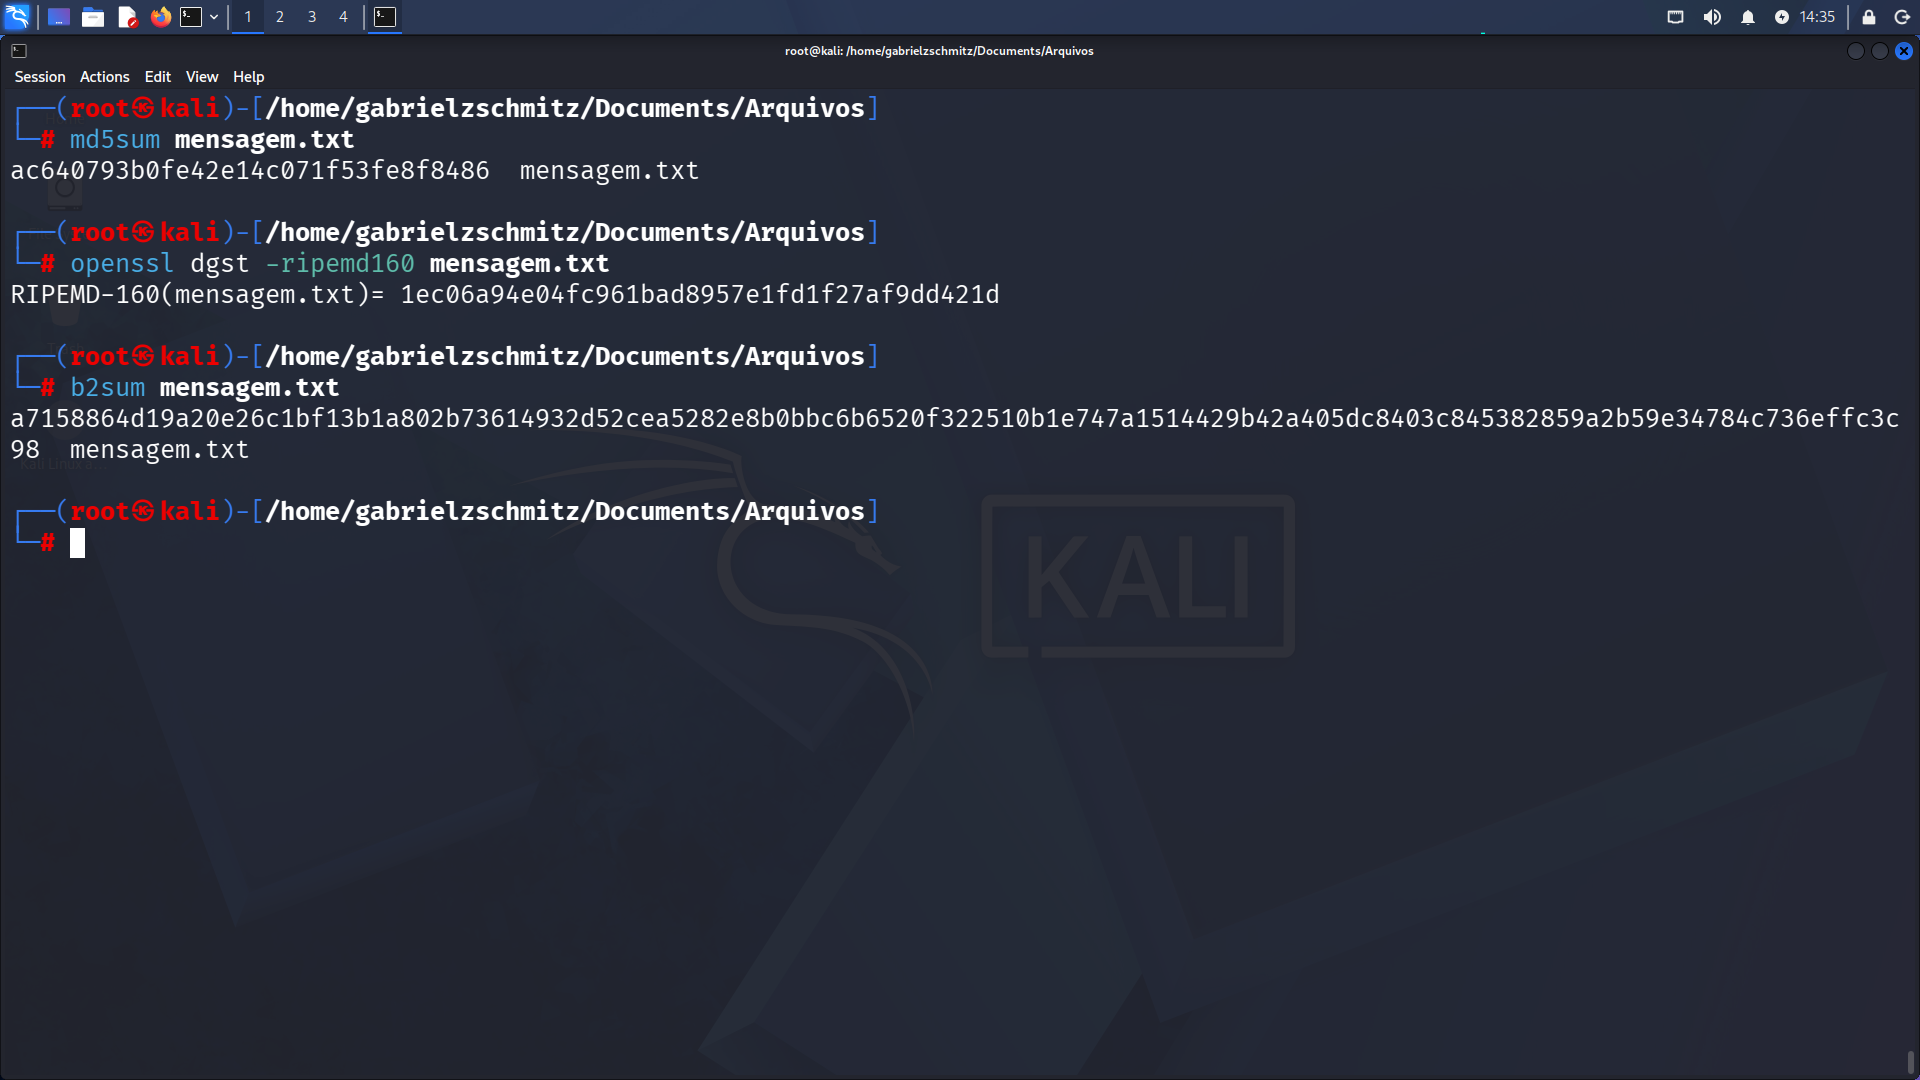
\includegraphics[width=0.99\textwidth]{./fig/fig8.6.png}
  \caption{Cálculo do hash Blake2 do arquivo mensagem.txt}
  \label{fig:fig8.6}
\end{figure}

\newpage

\question[Atividade 8.7]{Cálculo de Hash SHA-1, SHA-512 e SHA3-512}

\begin{figure}[H]
  \centering
  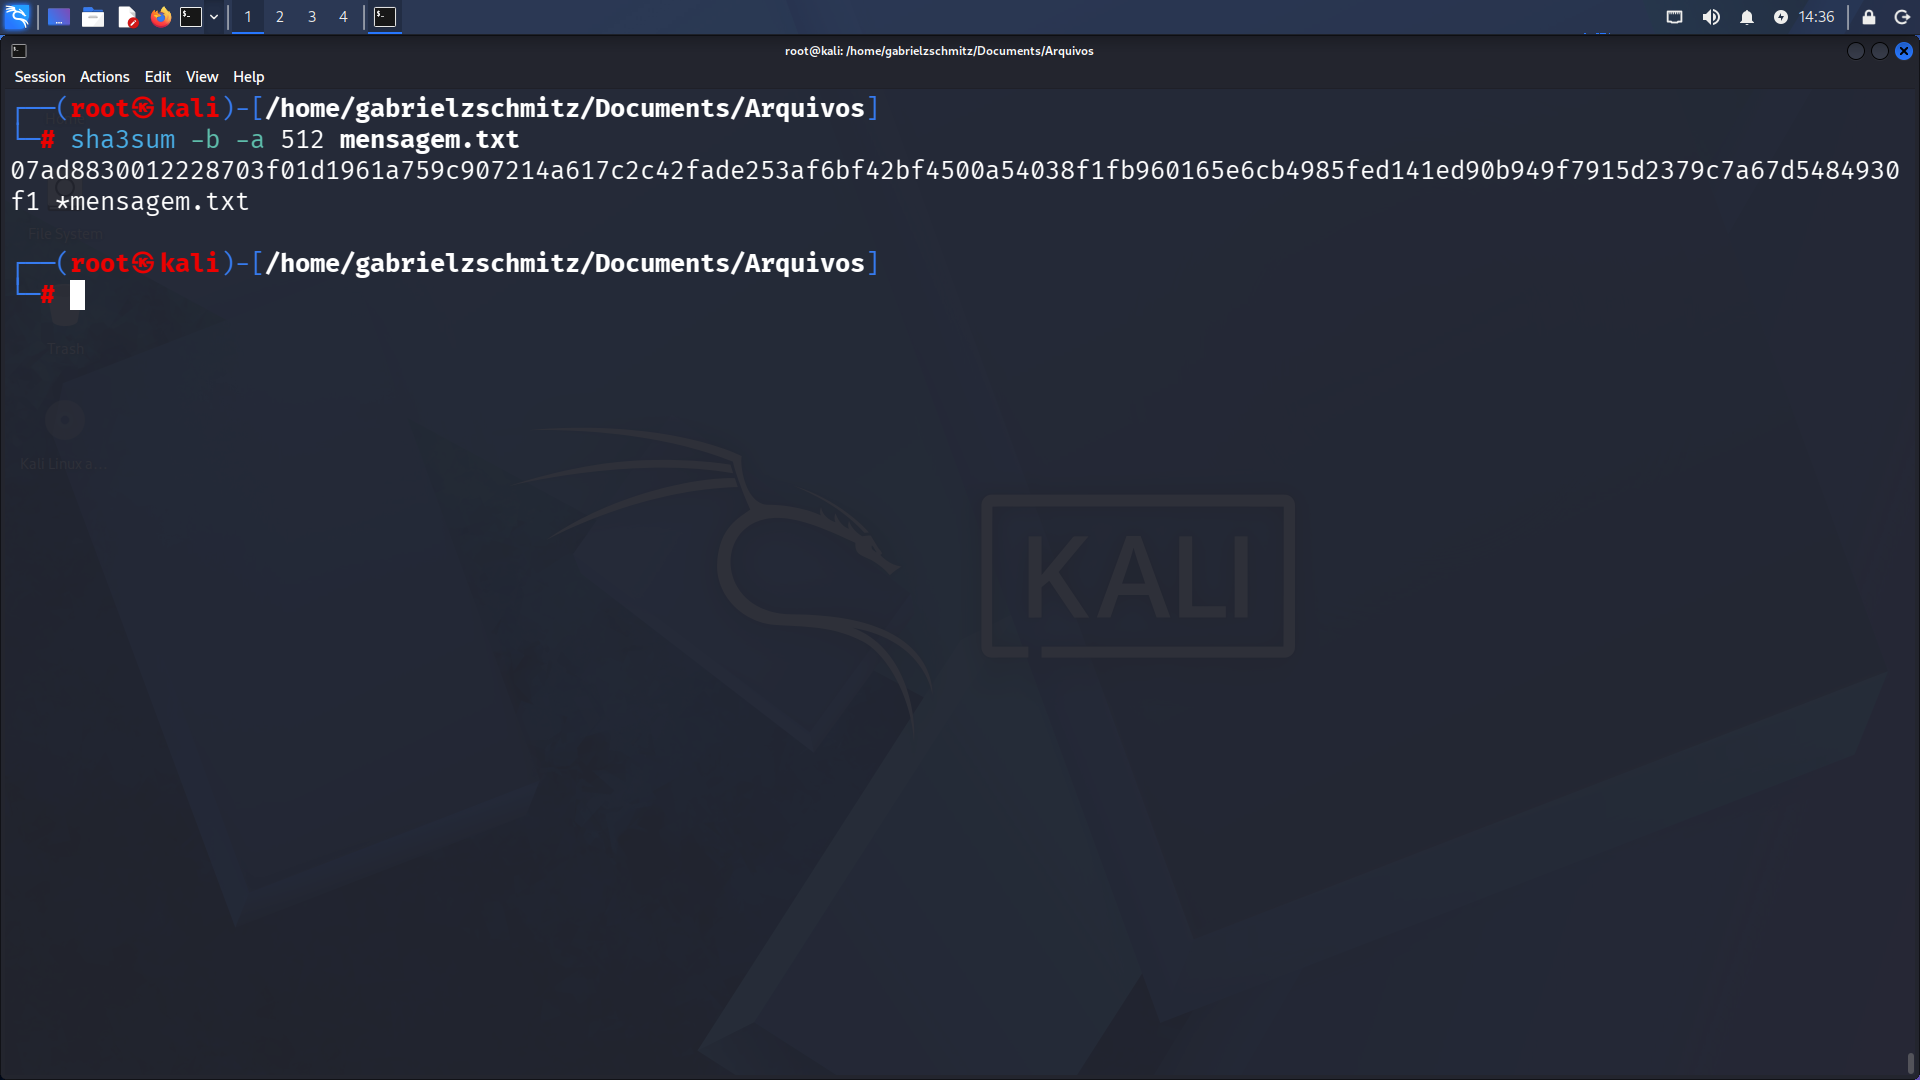
\includegraphics[width=0.99\textwidth]{./fig/fig8.7.png}
  \caption{Cálculo do hash SHA3-512 do arquivo mensagem.txt}
  \label{fig:fig8.7}
\end{figure}

\newpage

\question[Atividade 8.8]{Criptografia Assimétrica com RSA-2048}

\begin{figure}[H]
  \centering
  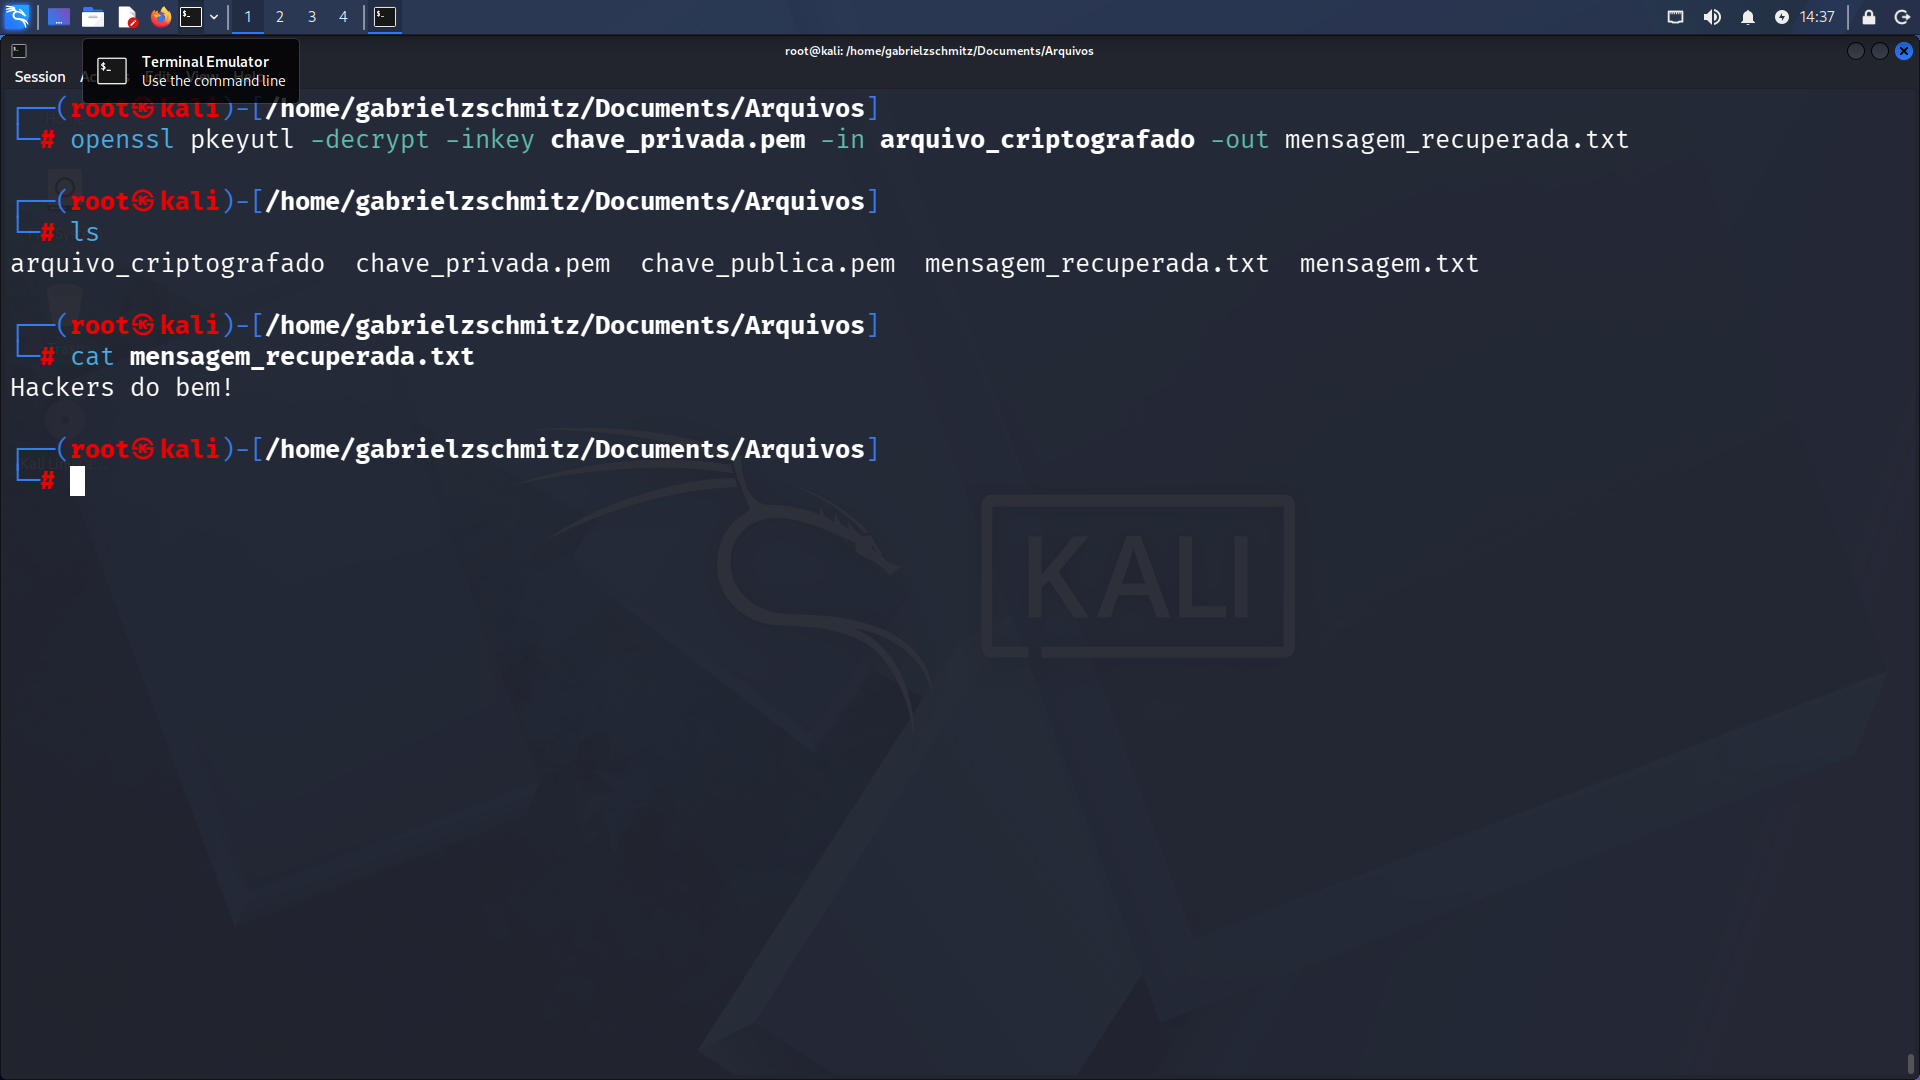
\includegraphics[width=0.99\textwidth]{./fig/fig8.8.png}
  \caption{Recuperação do conteúdo original após descriptografia com RSA}
  \label{fig:fig8.8}
\end{figure}

\newpage

\question[Atividade 8.9]{Criptografia Híbrida utilizando ECC-256 e AES-256}

\begin{figure}[H]
  \centering
  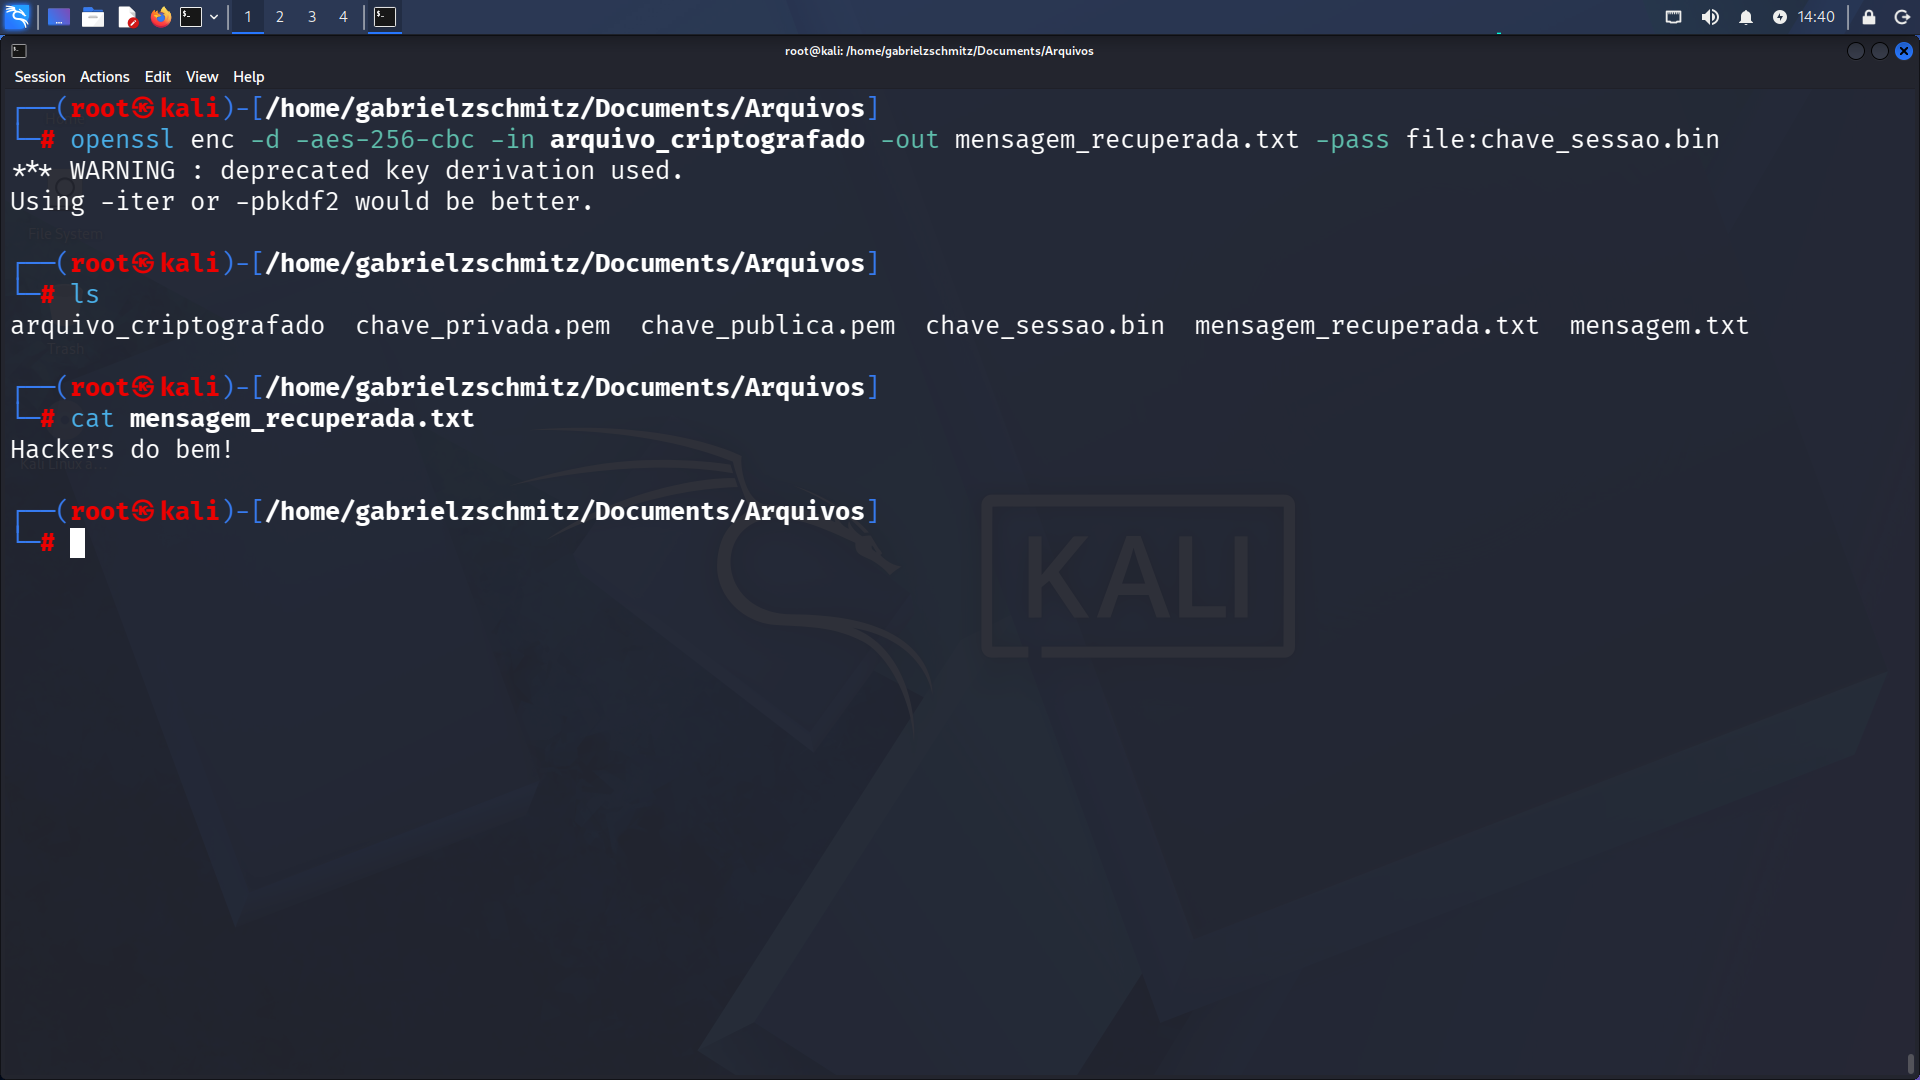
\includegraphics[width=0.99\textwidth]{./fig/fig8.9.png}
  \caption{Recuperação do arquivo original utilizando criptografia híbrida ECC e AES}
  \label{fig:fig8.9}
\end{figure}

\newpage

\question[Atividade 8.10]{Assinatura Digital com RSA-2048}

\begin{figure}[H]
  \centering
  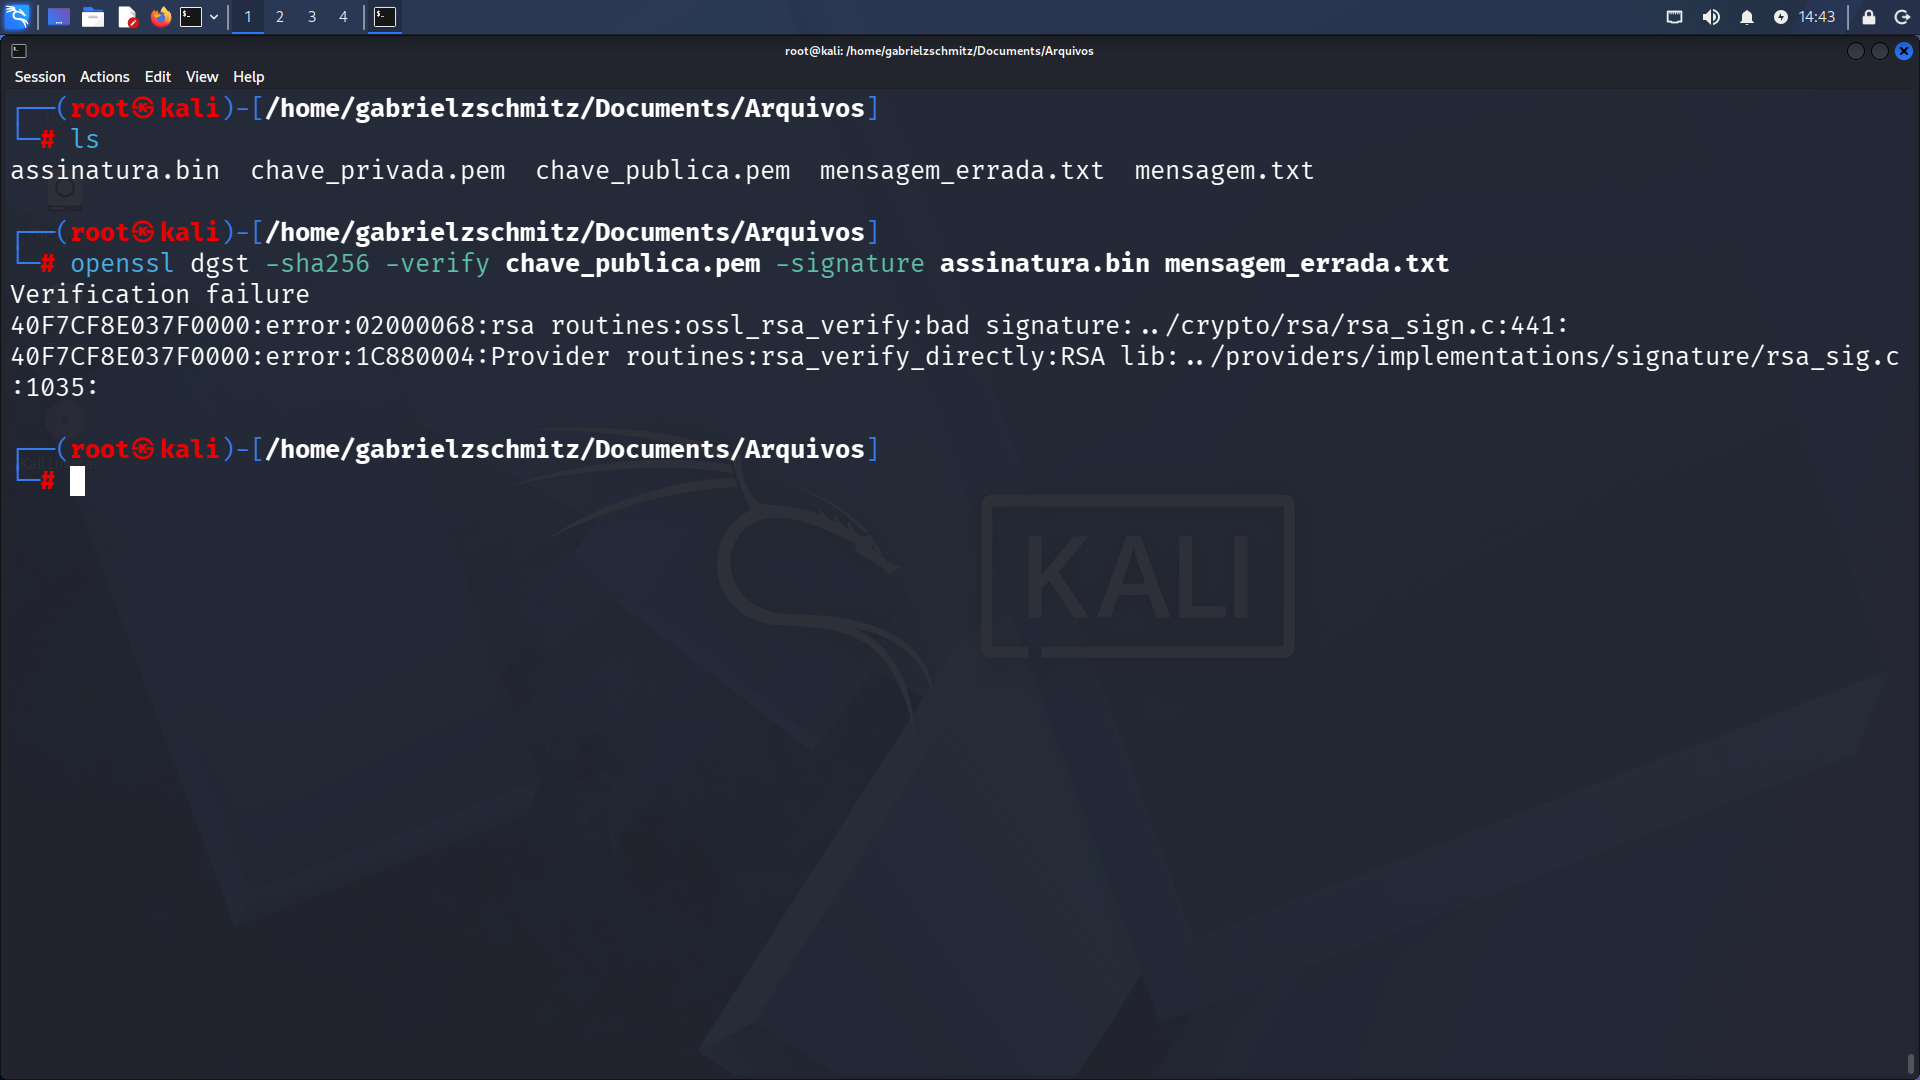
\includegraphics[width=0.99\textwidth]{./fig/fig8.10.png}
  \caption{Falha na verificação da assinatura digital após alteração do arquivo}
  \label{fig:fig8.10}
\end{figure}
